%!TEX root = da2020-09.tex

\Chapter{9}{Round Elimination}

\noindent
In this chapter we introduce the basic idea of a proof technique, called \emph{round elimination}.
Round elimination is based on the following idea. Assume that there exists a distributed algorithm $S_0$ with complexity $T$ solving a problem $\Pi_0$. Then there exists a distributed algorithm $S_1$ with complexity $T-1$ for solving another problem $\Pi_1$. That is, if we can solve problem $\Pi_0$ in $T$ communication rounds, then we can solve a related problem $\Pi_1$ exactly one round faster\mydash we can ``eliminate one round''. If this operation is repeated $T$ times, we end up with some algorithm $S_T$ with round complexity $0$ for some problem $\Pi_T$. If $\Pi_T$ is not a \emph{trivial} problem, that is, cannot be solved in $0$ rounds, we have reached a contradiction: therefore the assumption that $\Pi_0$ can be solved in $T$ rounds has to be wrong. This is a very useful approach, as it is much easier to reason about $0$-round algorithms than about algorithms in general.

\section{Bipartite Model and Biregular Trees}

When dealing with round elimination, we will consider a model that is a variant of the $\PN$ model from Chapter~\chapterref{3}. We will restrict our attention to specific families of graphs (see Figure~\ref{fig:biregular}):
\begin{enumerate}
	\item \textbf{Bipartite.} The set of nodes $V$ is partitioned into two sets: the \emph{active} nodes $V_A$ and the \emph{passive} nodes $V_P$. The partitioning forms a proper $2$-coloring of the graph, i.e., each edge connects an active node with a passive node. The role of a node\mydash active or passive\mydash is part of the local input.
	\item \textbf{Biregular trees.} We will assume that the input graphs are \emph{biregular} trees: the graph is connected, there are no cycles, each node in $V_A$ has degree $d$ or 1, and each node in $V_P$ has degree $\delta$ or 1. We say that such a tree is $(d,\delta)$-biregular. See Figure~\ref{fig:biregular} for an illustration.
\end{enumerate}

\begin{figure}
	\centering
	\includegraphics[page=\PBipartiteModel,scale=0.33]{figs.pdf}
	\caption{The bipartite model; black nodes are active and white nodes are passive. (a)~A $(3,3)$-biregular tree. (b)~A $(3,2)$-biregular tree.} \label{fig:biregular}
\end{figure}

\subsection{Bipartite Locally Verifiable Problem}

We consider a specific family of problems, called \emph{bipartite locally verifiable} problems. Such a problem is defined as a 3-tuple $\Pi = (\Sigma, \collA, \collP)$, where:
\begin{itemize}
	\item $\Sigma$ is a finite alphabet.
	\item $\collA$ and $\collP$ are finite collections of multisets, where each multiset $A \in \collA$ and $P \in \collP$ consists of a finite number of elements from $\Sigma$. These are called the \emph{active} and \emph{passive configurations}. 
\end{itemize}
Recall that multisets are sets that allow elements to be repeated. We use the notation $[x_1, x_2, \dotsc, x_k]$ for a multiset that contains $k$ elements; for example, $[1,1,2,2,2]$ is a multiset with two $1$s and three $2$s. Note that the order of elements does not matter, for example, $[1,1,2] = [1,2,1] = [2,1,1]$.

In problem $\Pi$, each active node $v \in V_A$ must label its incident $\deg(v)$ edges with elements of $\Sigma$ such that the labels of the incident edges, considered as a multiset, form an element of $\collA$. The order of the labels does not matter. The passive nodes do not have outputs. Instead, we require that for each passive node the labels of its incident edges, again considered as a multiset, form an element of $\collP$. A labeling $\varphi\colon E \to \Sigma$ is a solution to $\Pi$ if and only if the incident edges of all active and passive nodes are labeled according to some configuration.

In this chapter we will only consider labelings such that all nodes of degree 1 accept any configuration: these will not be explicitly mentioned in what follows. Since we only consider problems in $(d,\delta)$-biregular trees, each active configuration will have $d$ elements and each passive configuration $\delta$ elements.

\subsection{Examples} \label{ssec:bipartite-examples}

To illustrate the definition of bipartite locally verifiable labelings, we consider some examples (see Figure~\ref{fig:bipartite-problem-examples}).

\begin{figure}
	\centering
	\includegraphics[page=\PBipartiteModelExamples,scale=0.3]{figs.pdf}
	\caption{Bipartite locally verifiable labeling problems. (a)~$5$-edge coloring in a $(3,3)$-biregular tree. (b)~Maximal matching in a $(3,3)$-biregular tree. (c)~Sinkless orientation in a $(3,3)$-biregular tree. (d)~Weak 3-labeling in a $(3,2)$-biregular tree.} \label{fig:bipartite-problem-examples}
\end{figure}

\paragraph{Edge Coloring.} A $c$-edge coloring is an assignment of labels from $\{1,2,\dotsc,c\}$ to the edges such that no node has two incident edges with the same label. 

Consider the problem of $5$-edge coloring $(3,3)$-biregular trees. The alphabet $\Sigma$ consists of the five edge colors $\{ 1, 2, 3, 4, 5 \}$. The active configurations consist of all multisets of three elements $[x,y,z]$, such that all elements are distinct and come from $\Sigma$. The problem is symmetric, and the passive configurations consist of the same multisets:
\[
\begin{split}
	\collA = \collP = \bigl\{\,
		&[1,2,3],\,
		[1,2,4],\,
		[1,2,5],\,
		[1,3,4],\,
		[1,3,5], \\
		&[1,4,5],\,
		[2,3,4],\,
		[2,3,5],\,
		[2,4,5],\,
		[3,4,5]
	\,\bigr\}.
\end{split}
\]

\paragraph{Maximal Matching.} A maximal matching $M$ is a subset of the edges such that no two incident edges are in $M$ and no edge can be added to~$M$.

Consider maximal matching on $(3,3)$-biregular trees. To encode a matching, we could use just two labels: $\mM$ for matched and $\mU$ for unmatched. Such a labeling, however, has no way of guaranteeing maximality. We use a third label $\mP$, called a pointer:
\[
	\Sigma = \{ \mM, \mP, \mU \}.
\]
The active nodes either output $[ \mM, \mU, \mU ]$, denoting that the edge marked $\mM$ is in  the matching, or they output $[\mP, \mP, \mP]$, denoting that they are unmatched, and thus all passive neighbors \emph{must} be matched with another active node:
\[
	\collA = \bigl\{\, [ \mM, \mU, \mU ], \, [\mP, \mP, \mP] \, \bigr\}.
\]
Passive nodes must verify that they are matched with at most one node, and that if they have an incident label $\mP$, then they also have an incident label $\mM$ (to ensure maximality). Hence the passive configurations are
\[
	\collP = \bigl\{\,
		[ \mM, \mP, \mP ],\,
		[ \mM, \mP, \mU ],\,
		[ \mM, \mU, \mU ],\,
		[ \mU, \mU, \mU ]
	\,\bigr\}.
\]

\paragraph{Sinkless Orientation.} A \emph{sinkless orientation} is an orientation of the edges such that each node has an edge oriented away from it. That is, no node is a \emph{sink}. We will consider here sinkless orientation in (3,3)-biregular trees; leaf nodes can be sinks, but nodes of degree $3$ must have at least one outgoing edge.

To encode sinkless orientation, each active node chooses an orientation of its incident edges: outgoing edges are labeled $\mO$ and incoming edges $\mI$. Thus the alphabet is $\Sigma = \{ \mO, \mI \}$. Each node must have an outgoing edge, so the active configurations are all multisets that contain at least one $\mO$:
\[
	\collA = \bigl\{ [\mO, x, y] \bigm| x, y \in \Sigma \bigr\}.
\]
The passive configurations are similar, but the roles of the labels are reversed: an outgoing edge for an active node is an incoming edge for a passive node. Therefore each passive node requires that at least one of its incident edges is labeled $\mI$, and the passive configurations are
\[
	\collP = \bigl\{ [\mI, x, y] \bigm| x, y \in \Sigma \bigr\}.
\]

\paragraph{Weak Labeling.} We will use the following problem as the example in the remainder of this chapter. Consider $(3,2)$-biregular trees. A \emph{weak $3$-labeling} is an assignment of labels from the set $\{1,2,3\}$ to the edges such that each active node has at least two incident edges labeled with different labels. Each passive node must have its incident edges labeled with the same label. The problem can be formalized as
\begin{align*}
	\Sigma &= \{1,2,3\}, \\
	\collA &= \bigl\{\,
		[ 1, 1, 2 ],\,
		[ 1, 1, 3 ],\,
		[ 1, 2, 2 ],\,
		[ 1, 2, 3 ],\,
		[ 1, 3, 3 ],\,
		[ 2, 2, 3 ],\,
		[ 2, 3, 3 ]
	\,\bigr\}, \\
	\collP &= \bigl\{\,
		[ 1, 1 ],\,
		[ 2, 2 ],\,
		[ 3, 3 ]
	\,\bigr\}. 
\end{align*}

\section{Introducing Round Elimination}

Round elimination is based on the following basic idea. Assume that we can solve some bipartite locally verifiable problem $\Pi_0$ in $T$ communication rounds on $(d,\delta)$-biregular trees. Then there exists a bipartite locally verifiable problem $\Pi_1$, called the \emph{output problem} of $\Pi_0$, that can be solved in $T-1$ rounds on $(\delta,d)$-biregular trees. The output problem is uniquely defined, and we refer to the output problem of $\Pi$ as $\re(\Pi)$. The definition of output problem will be given in Section~\ref{ssec:output-problems}.

A single round elimination step is formalized in the following lemma.

\begin{lemma}[Round elimination lemma] \label{lem:round-elimination}
	Let $\Pi$ be bipartite locally verifiable problem that can be solved in $T$ rounds in $(d,\delta)$-biregular trees. Then the output problem $\re(\Pi)$ of $\Pi$ can be solved in $T-1$ rounds in $(\delta,d)$-biregular trees.
\end{lemma}

\subsection{Impossibility Using Iterated Round Elimination}
Lemma~\ref{lem:round-elimination} can be iterated, applying it to the output problem of the previous step. This will yield a sequence of $T+1$ problems
\[
	\Pi_0 \rightarrow \Pi_1 \rightarrow \cdots \rightarrow \Pi_{T},
\]
where $\Pi_{i+1} = \re(\Pi_i)$ for each $i = 0, 1, \dotsc, T-1$.

If we assume that there is a $T$-round algorithm for $\Pi_0$, then by an iterated application of Lemma~\ref{lem:round-elimination}, there is a $(T-1)$-round algorithm for $\Pi_1$, a $(T-2)$-round algorithm for $\Pi_2$, and so on. In particular, there is a $0$-round algorithm for $\Pi_T$.

Algorithms that run in $0$ rounds are much easier to reason about than algorithms in general. Since there is no communication, each active node must simply map its input, essentially its degree, to some output. In particular, we can try to show that there is no 0-round algorithm for $\Pi_T$. If this is the case, we have a contradiction with our original assumption: there is no $T$-round algorithm for $\Pi_0$.

We will now proceed to formally define output problems.

\subsection{Output Problems} \label{ssec:output-problems}

For each locally verifiable problem $\Pi$ we will define a unique \emph{output problem} $\re(\Pi)$.

Let $\Pi_0 = (\Sigma_0, \collA_0, \collP_0)$ be a bipartite locally verifiable problem on $(d,\delta)$-biregular trees. We define the output problem $\Pi_1 = \re(\Pi_0) = (\Sigma_1, \collA_1, \collP_1)$ of $\Pi_0$ on $(\delta,d)$-biregular trees as follows\mydash note that we swapped the degrees of active vs.\ passive nodes here.

The alphabet $\Sigma_1$ consists of all possible non-empty subsets of $\Sigma_0$. The roles of the active and passive nodes are inverted, and new configurations are computed as follows.
\begin{enumerate}
	\item The active configurations $\collA_1$ consist of all multisets
	\[
	[ X_1, X_2, \dotsc, X_{\delta} ], \text{ where } X_i \in \Sigma_1 \text{ for all } i = 1,\dotsc,\delta,
	\] 
	such that for \textbf{\emph{every}} choice of $x_1 \in X_1$, $x_2 \in X_2$, \ldots, $x_{\delta} \in X_{\delta}$ we have $[x_1, x_2, \dotsc, x_{\delta}] \in \collP_0$, i.e., it is a passive configuration of $\Pi_0$.
	\item The passive configurations $\collP_1$ consist of all multisets
	\[
	[ Y_1,  Y_2, \dotsc, Y_d ], \text{ where } Y_i \in \Sigma_1 \text{ for all } i = 1,\dotsc,d,
	\]
	for which \textbf{\emph{there exists}} a choice $y_1 \in Y_1$, $y_2 \in Y_2$, \ldots, $y_d \in Y_d$ with $[ y_1, y_2, \dotsc, y_d] \in \collA_0$, i.e., it is an active configuration of $\Pi_0$.
\end{enumerate}

\subsection{Example: Weak 3-labeling} \label{ssec:example-w3ec}

To illustrate the definition, let us construct the output problem $\re(\Pi_0) = (\Sigma_1, \collA_1, \collP_1)$ of weak 3-labeling problem $\Pi_0 = (\Sigma_0, \collA_0, \collP_0)$. Recall that
\begin{align*}
	\Sigma_0 &= \{ 1,2,3 \}, \\
	\collA_0 &= \bigl\{\,
		[ 1, 1, 2 ],\,
		[ 1, 1, 3 ],\,
		[ 1, 2, 2 ],\,
		[ 1, 2, 3 ],\,
		[ 1, 3, 3 ],\,
		[ 2, 2, 3 ],\,
		[ 2, 3, 3 ]
	\,\bigr\}, \\
	\collP_0 &= \bigl\{\,
		[ 1, 1 ],\,
		[ 2, 2 ],\,
		[ 3, 3 ]
	\,\bigr\}. 
\end{align*}
The alphabet $\Sigma_1$ consists of all possible (non-empty) subsets of $\Sigma_0$: 
\[
	\Sigma_1 = \bigl\{ \{ 1 \}, \{ 2 \}, \{ 3 \}, \{ 1, 2 \}, \{ 1, 3 \}, \{ 2, 3 \}, \{ 1, 2, 3 \} \bigr\}.
\]
The active configurations $\collA_1$ are all multisets $[ X,Y ]$ with $X, Y \in \Sigma_1$ such that \emph{all} choices of elements $x \in X$ and $y \in Y$ result in a multiset $[x,y] \in \collP_0$. For example $X = \{1\}$ and $Y = \{1,2\}$ is \emph{not} a valid choice: we could choose $x = 1$ and $y = 2$ to construct $[1,2] \notin \collP_0$. In general, whenever $|X| > 1$ or $|Y| > 1$, we can find $x \in X$, $y \in Y$ with $x \ne y$, and then $[x,y] \notin \collP_0$. Therefore the only possibilities are $|X| = |Y| = 1$, and then we must also have $X = Y$. We obtain
\[ 
\collA_1 = \Bigl\{\, \bigl[\{ 1 \}, \{1 \}\bigr],\, \bigl[\{ 2 \}, \{2 \}\bigr],\, \bigl[\{ 3 \}, \{3 \}\bigr] \,\Bigr\}. 
\] 
But since the active configurations only allow singleton sets, we can restrict ourselves to them when listing the possible passive configurations; we obtain simply
\[
\begin{split}
	\collP_1 = \Bigl\{\,
		&\bigl[ \{1\}, \{1\}, \{2\} \bigr],\,
		\bigl[ \{1\}, \{1\}, \{3\} \bigr],\,
		\bigl[ \{1\}, \{2\}, \{2\} \bigr],\,
		\bigl[ \{1\}, \{2\}, \{3\} \bigr],\\[-2pt]
		&\bigl[ \{1\}, \{3\}, \{3\} \bigr],\,
		\bigl[ \{2\}, \{2\}, \{3\} \bigr],\,
		\bigl[ \{2\}, \{3\}, \{3\} \bigr]
	\,\Bigr\}.
\end{split}
\]

\subsection{Complexity of Output Problems}

In this section we prove Lemma~\ref{lem:round-elimination} that states that the output problem $\re(\Pi)$ of $\Pi$ can be solved one round faster than $\Pi$. 

The proof is by showing that we can truncate the execution of a $T$-round algorithm and output the set of \emph{possible outputs}. As we will see, this is a solution to the output problem.

\begin{proof}[Proof of Lemma~\ref{lem:round-elimination}]
	Assume that we can solve some problem $\Pi_0 = (\Sigma_0, \collA_0, \collP_0)$ on $(d,\delta)$-biregular trees in $T$ rounds using some deterministic $\PN$-algorithm $S$. We want to design an algorithm that works in $(\delta,d)$-biregular trees and solves $\Pi_1 = \re(\Pi_0)$ in $T-1$ rounds.
	
	Note that we are considering the same family of networks, but we are only switching the sides that are marked as active and passive. We will call these \emph{$\Pi_0$-active} and \emph{$\Pi_1$-active} sides, respectively.
	
	The algorithm for solving $\Pi_1$ works as follows. Let $N = (V,P,p)$ be any port-numbered network with a $(\delta,d)$-biregular tree as the underlying graph. Each $\Pi_1$-active node $u$, in $T-1$ rounds, gathers its full $(T-1)$-neighborhood $\ball_N(u, T-1)$. Now it considers all \emph{possible} outputs of its $\Pi_0$-active neighbors under the algorithm $S$, and outputs these.
	
	Formally, this is done as follows. When $N$ is a port-numbered network, we use $\ball_{N}(u,r)$ to refer to the information within distance $r$ from node $u$, including the local inputs of the nodes in this region, as well as the port numbers of the edges connecting nodes within this region. We say that a port-numbered network $H$ is \emph{compatible} with $\ball_{N}(u,r)$ if there is a node $v \in H$ such that $\ball_{H}(v,r)$ is isomorphic to $\ball_{N}(u,r)$.

	For each neighbor $v$ of $u$, node $u$ constructs all possible fragments $\ball_{H}(v, T)$ such that $H$ is compatible with $\ball_N(u,T-1)$ and has a $(\delta,d)$-biregular tree as its underlying graph. Then $u$ simulates the $\Pi_0$-algorithm $S$ on $\ball_{H}(v,T)$. The algorithm outputs some label $x \in \Sigma_0$ on the edge $\{u,v\}$. Node $u$ adds each such label $x$ to set $S(u,v)$; finally node $u$ will label edge $\{u,v\}$ with $S(u,v)$.
	
	\begin{figure}
		\centering
		\includegraphics[page=\PRoundElimination,scale=0.3]{figs.pdf}
		\caption{Illustration of the round elimination step. A fragment of a $(2,3)$-biregular tree. The 3-neighborhood of node $u$ consists of the gray area. The 4-neighborhoods of nodes $v$ and $w$ consist of the blue and orange areas, respectively. Since the input is a tree, these intersect exactly in the 3-neighborhood of $u$.} \label{fig:round-elimination}
	\end{figure}
	
	By construction, $S(u,v)$ is a nonempty set of labels from $\Sigma_0$, i.e., $S(u,v) \in \Sigma_1$. We now prove that the sets $S(u,v)$ form a solution to $\Pi_1$. We use the assumption that the underlying graph $G$ is a tree. Let $H$ be any port-numbered network compatible with $\ball_{N}(u,T-1)$. Consider any two neighbors $v$ and $w$ of $u$: since there are no cycles, we have
	\[\ball_{H}(v,T) \cap \ball_{H}(w,T) = \ball_{H}(u,T-1) = \ball_{N}(u,T-1).\]
	In particular, once $\ball_{H}(u,T-1)$ is fixed, the outputs of $v$ and $w$, respectively, depend on the structures of $\ball_{H}(v,T) \setminus \ball_{H}(u,T-1)$ and $\ball_{H}(w,T) \setminus \ball_{H}(u,T-1)$, which are completely distinct. See Figure~\ref{fig:round-elimination} for an illustration. Therefore, if there exist $x \in S(u,v)$ and $y \in S(u,w)$, then there exists a port-numbered network $H$ such that running $S$, node $v$ outputs $x$ on $\{v,u\}$ and node $w$ outputs $y$ on $\{ w,u \}$. This further implies that since $S$ is assumed to work correctly on all port-numbered networks, for any combination of $x_1 \in S(u,v_1)$, $x_2 \in S(u,v_2)$, \ldots, $x_{\delta} \in S(u,v_{\delta})$, we must have that \[[x_1, x_2, \dots, x_{\delta}] \in \collP_0.\] This implies that
	\[
		[S(u,v_1),\, S(u,v_2),\, \dotsc,\, S(u, v_{\delta})] \in \collA_1.
	\]
	
	It remains to show that for each $\Pi_0$-active node $v$, it holds that the sets $S(u_1, v)$, $S(u_2, v)$, \ldots, $S(u_d, v)$, where $u_i$ are neighbors of $v$, form a configuration in $\collP_1$. To see this, note that the $\Pi_1$-active nodes $u_i$ simulate $S$ on every port-numbered fragment, including the true neighborhood $\ball_{N}(v,T)$ of $v$. This implies that the output of $v$ on $\{v,u_i\}$ running $S$ in network $N$ is included in $S(u_i, v)$. Since $S$ is assumed to be a correct algorithm, these true outputs $x_1 \in S(u_1, v)$, $x_2 \in S(u_2, v)$, \ldots, $x_{d} \in S(u_d,v)$ form a configuration \[[x_1, x_2, \dots, x_d] \in \collA_0,\] which implies that
	\[
		[S(u_1, v),\, S(u_2, v),\, \dots,\, S(u_d,v)] \in \collP_1,
	\] as required. 
\end{proof}

\subsection{Example: Complexity of Weak 3-labeling} \label{ssec:output-weak3}

Now we will apply the round elimination technique to show that the weak 3-labeling problem is not solvable in 1 round. To do this, we show that the output problem of weak 3-labeling is not solvable in 0 rounds.

\begin{lemma}
	Weak 3-labeling is not solvable in 1 round in the \PN-model on $(3,2)$-biregular trees.
\end{lemma}

\begin{proof}
	In Section~\ref{ssec:example-w3ec} we saw the output problem of weak 3-labeling. We will now show that this problem is not solvable in 0 rounds on $(2,3)$-biregular trees. By Lemma~\ref{lem:round-elimination}, weak 3-labeling is then not solvable in 1 round on $(3,2)$-biregular trees. Let $\Pi_1 = (\Sigma_1, \collA_1, \collP_1)$ denote the output problem of weak 3-labeling.
	
	In a 0-round algorithm an active node $v$ sees only its own side (active or passive) and its own port numbers. Since
	\[ 
	\collA_1 = \Bigl\{\, \bigl[\{ 1 \}, \{1 \}\bigr],\, \bigl[\{ 2 \}, \{2 \}\bigr],\, \bigl[\{ 3 \}, \{3 \}\bigr] \,\Bigr\},
	\] 
	each active node $v$ must output the same label $X \in \bigl\{ \{1\}, \{2\}, \{3\} \bigr\}$ on both of its incident edges.
	
	Since all active nodes look the same, they all label their incident edges with exactly one label $X$. Since $[X, X, X]$ is not in $\collP_1$ for any $X \in \Sigma_1$, we have proven the claim. 
\end{proof}

\subsection{Example: Iterated Round Elimination} \label{ssec:repeated}

We will finish this chapter by applying round elimination \emph{twice} to weak 3-labeling. We will see that the problem
\[
	\Pi_2 = \re(\Pi_1) = \re(\re(\Pi_0))
\]
obtained this way \emph{is} $0$-round solvable.

Let us first construct $\Pi_2$. Note that this is again a problem on $(3,2)$-biregular trees. We first \emph{simplify} notation slightly; the labels of $\Pi_1$ are sets and labels of $\Pi_2$ would be sets of sets, which gets awkward to write down. But the configurations in $\Pi_1$ only used \emph{singleton} sets. Therefore we can \emph{leave out} all non-singleton sets without changing the problem, and then we can \emph{rename} each singleton set $\{ x \}$ to $x$. After these simplifications, we have got
\begin{align*}
	\Sigma_1 &= \{ 1,2,3 \}, \\
	\collA_1 &= \bigl\{\,
		[ 1, 1 ],\,
		[ 2, 2 ],\,
		[ 3, 3 ]
	\,\bigr\}, \\ 
	\collP_1 &= \bigl\{\,
		[ 1, 1, 2 ],\,
		[ 1, 1, 3 ],\,
		[ 1, 2, 2 ],\,
		[ 1, 2, 3 ],\,
		[ 1, 3, 3 ],\,
		[ 2, 2, 3 ],\,
		[ 2, 3, 3 ]
	\,\bigr\}.
\end{align*}
Alphabet $\Sigma_2$ consists of all non-empty subsets of $\Sigma_1$, that is 
\[
	\Sigma_2 = \bigl\{ \{ 1 \}, \{ 2 \}, \{ 3 \}, \{ 1, 2 \}, \{ 1, 3 \}, \{ 2, 3 \}, \{ 1, 2, 3 \} \bigr\}.
\]
The active configurations are all multisets $[X_1, X_2, X_3]$ where $X_1,X_2,X_3 \in \Sigma_2$ such that \emph{any} way of choosing $x_1 \in X_1$, $x_2 \in X_2$, and $x_3 \in X_3$ is a configuration in $\collP_1$. There are many cases to check, the following observation will help here (the proof is left as Exercise~\ref{ex:pi2}):
\begin{itemize}
	\item $\collP_1$ consists of all $3$-element multisets over $\Sigma_1$ where at least one of the elements is not $1$, at least one of the elements is not $2$, and at least one of the elements is not $3$.
	\item It follows that $\collA_2$ consists of all $3$-element multisets over $\Sigma_2$ where at least one of the elements does not contain $1$, at least one of the elements does not contain $2$, and at least one of the elements does not contain $3$.
\end{itemize}
It follows that we can enumerate all possible configurations e.g.\ as follows (here $X,Y,Z \in \Sigma_2$):
\begin{equation}\label{eq:pi2}
\begin{split}
	\collA_2
	      = {} &\Bigl\{ \, \bigl[ X, Y, Z \bigr] \bigm| X \subseteq \{1, 2\}, Y \subseteq \{ 1, 3 \}, Z \subseteq \{ 2, 3 \} \,\Bigr\} \\
	{} \cup {} &\Bigl\{ \, \bigl[ X, Y, Z \bigr] \bigm| X \subseteq \{1\}, Y \subseteq \{ 2, 3 \}, Z \subseteq \{ 1, 2, 3 \} \,\Bigr\} \\
	{} \cup {} &\Bigl\{ \, \bigl[ X, Y, Z \bigr] \bigm| X \subseteq \{2\}, Y \subseteq \{ 1, 3 \}, Z \subseteq \{ 1, 2, 3 \} \,\Bigr\} \\
	{} \cup {} &\Bigl\{ \, \bigl[ X, Y, Z \bigr] \bigm| X \subseteq \{3\}, Y \subseteq \{ 1, 2 \}, Z \subseteq \{ 1, 2, 3 \} \,\Bigr\}.
\end{split}
\end{equation}
On the passive side, $\collP_2$ consists of all multisets $[X,Y]$ where we can choose $x \in X$ and $y \in Y$ with $[x,y] \in \collA_1$. But $[x,y] \in \collA_1$ is equivalent to $x = y$, and hence $\collP_2$ consists of all multisets $[X,Y]$ where we can choose some $x \in X$ and choose the same value $x \in Y$. Put otherwise,
\[
\collP_2 = \Bigl\{ \, \bigl[ X, Y \bigr] \bigm| X \in \Sigma_2,\, Y \in \Sigma_2,\, X \cap Y \ne \emptyset \,\Bigr\}.
\]

\begin{lemma}
	Let $\Pi_0$ denote the weak 3-labeling problem. The problem $\Pi_2 = \re(\re(\Pi_0)) = (\Sigma_2, \collA_2, \collP_2)$ is solvable in $0$ rounds.
\end{lemma}

\begin{proof}
	The active nodes always choose the configuration
	\[
	\bigl[\{ 1, 2 \}, \{ 1, 3 \}, \{ 2, 3 \} \bigr] \in \collA_2
	\]
	and assign the sets in some way using the port numbers, e.g., the edge incident to port $1$ is labeled with $\{2,3\}$, the edge incident to port $2$ is labeled with $\{1,3\}$, and the edge incident to port $3$ is labeled with $\{1,2\}$.

	Since each pair of these sets has a non-empty intersection, no matter which sets are assigned to the incident edges of passive nodes, these form a valid passive configuration in $\collP_2$.
\end{proof}

\section{Quiz}

Consider the following bipartite locally verifiable labeling problem $\Pi = (\Sigma, \collA, \collP)$ on $(2,2)$-biregular trees:
\begin{align*}
	\Sigma ={}& \{ 1, 2, 3, 4, 5, 6 \}, \\
	\collA ={}& \bigl\{\, [1, 6],\, [2, 5],\,[3, 4] \bigr\}, \text{ and} \\
	\collP ={}& \bigl\{\, [x, y] \bigm| x \in \{ 3, 5, 6 \}, y \in \{ 1, 2, 3, 4, 5, 6 \} \,\bigr\} \\
	  {}\cup{}& \bigl\{\, [x, y] \bigm| x \in \{4,5,6\}, y \in \{ 2, 3, 4, 5, 6 \} \,\bigr\}.
\end{align*}
Give a $0$-round algorithm for solving $\Pi$.

\section{Exercises}

\begin{ex}[encoding graph problems]\label{ex:encode-bipartite}
Even if a graph problem is defined for general (not bipartite) graphs, we can often represent it in the bipartite formalism. If we take a $d$-regular tree $G$ and subdivide each edge, we arrive at a $(d,2)$-biregular tree $H$, where the active nodes represent the nodes of $G$ and passive nodes represent the edges of $G$.

Use this idea to encode the following graph problems as bipartite locally verifiable labelings in $(d,2)$-biregular trees. Give a brief explanation of why your encoding is equivalent to the original problem. You can ignore the leaf nodes and their constraints; it is sufficient to specify constraints for the active nodes of degree $d$ and passive nodes of degree~$2$.
\begin{subex}[noitemsep]
	\item Vertex coloring with $d+1$ colors.
	\item Maximal matching.
	\item Dominating set.
	\item Minimal dominating set.
\end{subex}
\end{ex}

\begin{ex}[algorithms in the bipartite model]
	The bipartite model can be used to run algorithms from the standard $\PN$ and $\LOCAL$ models. Using the idea of Exercise~\ref{ex:encode-bipartite}, we encode the \emph{maximal independent set} problem in $3$-regular trees as the following bipartite locally verifiable problem $\Pi = (\Sigma, \collA, \collP)$ in $(3,2)$-biregular trees:
	\begin{align*}
		\Sigma &= \{ \mI, \mO, \mP \}, \\
		\collA &= \bigl\{ \, [\mI, \mI, \mI],\, [\mP, \mO, \mO] \, \bigr\}, \\
		\collP &= \bigl\{ \, [\mI, \mP],\, [\mI, \mO],\, [\mO, \mO] \, \bigr\}.
	\end{align*}
	In $\collA$, the first configuration corresponds to a node in the independent set $X$, and the second configuration to a node not in $X$. A node not in $X$ points to a neighboring active node with the label $\mP$: the node pointed to has to be in $X$. The passive configurations ensure that two active nodes connected by a passive node are not both in $X$, and that the pointer $\mP$ always points to a node in~$X$.
	
	Assume that the active nodes are given a 4-coloring $c$ as input. That is, $c\colon V_A \to \{1,2,3,4\}$ satisfies $c(v) \ne c(u)$ whenever the active nodes $v,u \in V_A$ share a passive neighbor $w \in V_P$. The nodes also know whether they are active or passive, but the nodes do not have any other information.
	
	Present a $\PN$-algorithm in the state machine formalism for solving~$\Pi$. Prove that your algorithm is correct. What is its running time? How does it compare to the complexity of solving maximal independent set in the $\PN$ model, given a $4$-coloring? 
\end{ex}

\begin{ex}[Round Eliminator]
	There is a computer program, called Round Eliminator, that implements the round elimination technique and that you can try out in a web browser:
	\begin{center}
		\url{https://github.com/olidennis/round-eliminator}
	\end{center}
	Let $\Pi_0$ be the weak 3-labeling problem defined in Section~\ref{ssec:bipartite-examples}. Use the Round Eliminator to find out what are $\Pi_1 = \re(\Pi_0)$ and $\Pi_2 = \re(\Pi_1)$. In your answer you need to show how to encode $\Pi_0$ in a format that is suitable for the Round Eliminator, what were the answers you got from the Round Eliminator, and how to turn the answers back into our usual mathematical formalism.
\end{ex}

\begin{ex}[iterated round elimination]\label{ex:pi2}
	Fill in the missing details in Section~\ref{ssec:repeated} to show that formula \eqref{eq:pi2} is a correct definition of the active configurations for problem $\Pi_2$ (i.e., it contains all possible configurations and only them).
\end{ex}

\begin{ex}[solving weak 3-labeling]
	Present a 2-round deterministic $\PN$-algorithm for solving weak 3-labeling in $(3,2)$-biregular trees.
\end{ex}

\begin{ex}[sinkless orientation]
	Consider the sinkless orientation problem, denoted by $\Pi$, on $(3,3)$-biregular trees from Section~\ref{ssec:bipartite-examples}. Compute the output problems $\re(\Pi)$ and $\re(\re(\Pi))$; include a justification for your results.
\end{ex}

\section{Bibliographic Notes}

Linial's \cite{linial92locality} lower bound for vertex coloring in cycles already used a proof technique that is similar to round elimination. However, for a long time it was thought that this is an ad-hoc technique that is only applicable to this specific problem. This started to change in 2016, when the same idea found another very different application \cite{brandt16lll}. Round elimination as a general-purpose technique was defined and formalized by Brandt~\cite{Brandt2019automatic} in 2019, and implemented as a computer program by Olivetti~\cite{Olivetti2019}.
